\section{Введение}

\textbf{Цель работы:}
1) измерение объемов форвакуумной и высоковакуумной частей установки; 2) определение скорости откачки системы в стационарном режиме, а также по ухудшению и по улучшению вакуума.

\textbf{В работе используются:}
вакуумная установка с манометрами: масляным, термопарным и ионизационным.

\subsection{Экспериментальная установка}
По степени разрежения вакуумные установки принято делить
на три класса: 1) низковакуумные -- до $10^{-2}$-$10^{-3}$ торр; 2) высоковакуумные -- $10^{-4}$-$10^{-7}$ торр; 3) установки сверхвысокого вакуума -- $10^{-8}$-$10^{-11}$ торр. В данной работе изучаются традиционные методы откачки механическим форвакуумным насосом до давления $10^{-2}$ торр и диффузионным масляным насосом до давления
$10^{-5}$ торр, а также методы измерения вакуума в этом диапазоне.

\begin{figure*}[h]
    \centering
    \includegraphics*[width = \linewidth]{p1.png}
    \caption{Схема эксперментальной установки}
    \label{pic:p1}
\end{figure*}

Установка изготовлена из стекла
и состоит из форвакуумного баллона (ФБ), высоковакуумного диффузионного насоса (ВН), высоковакуумного баллона (ВБ), масляного (М) и ионизационного (И) манометров, термопарных манометров
(М1 и M2), форвакуумного насоса (ФН) и соединительных кранов К1,
К2, ..., К6 (рис. 1). Кроме того, в состав установки входят: вариатор
(автотрансформатор с регулируемым выходным напряжением), или
реостат и амперметр для регулирования тока нагревателя диффузионного насоса.

Все краны вакуумной установки стеклянные. Стенки кранов тонкие, пробки кранов полые и составляют одно целое с рукоятками. Пробки кранов притерты к корпусам. Для герметизации используется вакуумная смазка.

Устройство и принцип действия \textit{форвакуумного насоса} схематически, но довольно ясно изображены на рис 2. В положениях <<а>> и <<б>> пластина <<А>> засасывает разреженный воздух из откачиваемого объёма, а пластина <<Б>> вытесняет ранее захваченный воздух в атмосферу. В положениях <<в>> и <<г>> пластины поменялись ролями.
\begin{figure*}[h]
    \centering
    \includegraphics*[width = 0.75\linewidth]{p2.png}
    \caption{Схема ротационного двухпластинчатого форвакуумного насоса}
    \label{pic:p2}
\end{figure*}

Устройство и принцип действия \textit{диффузионного насоса} схематически изображены на рис. 2. Такой насос работает в тысячи раз быстрее форвакуумного. Его действие основано на диффузии. Масло, налитое в сосуд А, подогревается электрической печкой. Пары масла поднимаются по трубке Б и вырываются из сопла В. Струя паров увлекает молекулы газа, которые поступают из откачиваемого сосуда через трубку ВВ. В трубке Г мало осаждается и стекает вниз. Оставшийся газ, выходя в трубку ФВ, откачивается форвакуумным насосом.

Диффузионный насос работает наиболее эффективно, когда длина свободного пробега молекул примерно равна ширине кольцевого зазора между соплом В и стенками трубки ВВ. Давление насыщенных паров масла при рабочей температуре, создаваемой обогревателем сосуда А, много больше $5\cdot 10^{-2}$ торр, поэтому пары масла создают плотную струю, увлекающую с собой молекулы газа.

Диффузионный насос, используемый в нашей установке (см. рис 1) имеет две ступени и соответственно два сопла. Одно сопло вертикальное (первая ступень), второе горизонтальное (вторая ступень). За второй ступенью имеется ещё одна печь, но пар из этой печи поступает не в сопло, а по тонкой трубке подводится ближе к печке первой ступени. Эта печь осуществляет фракционирование масла. Легколетучие фракции масла, испаряясь, поступают в первую ступень, обогащая её. По этой причине плотность струи первой ступени выше, и эта ступень начинает откачивать при более высоком давлении в форвакуумной части. Вторая ступень обогащается малолетучими фракциями масла. Плотность струи второй ступени меньше, но меньше и давление насыщенных паров. Соответственно, в откачиваемый объем поступает меньше паров масла, и его удаётся откачать до более высокого вакуума.

\textit{Термопарный манометр.} Чувствительным элементом манометра является платиново-родиевая термопара, спаянная с никелевой нитью накала и заключённая в стеклянный баллон. По нити накала НН пропускается ток постоянной величины. Для установки тока служит потенциометр R, расположенный на передней панели вакуумметра. Термопара ТТ присоединяется к милливольтметру, показания которого определяются температурой нити накала и зависят от отдачи тепла в окружающее пространство.

Потери тепла определяются теплопроводностью нити и термопары, теплопроводностью газа, переносом тепла конвективными потоками газа внутри лампы, и теплоизлучением нити (инфракрасное тепловое излучение). В обычном режиме лампы основную роль играет теплопроводность газа. При давлениях, не меньших 1 торр, теплопроводность газа, а вместе с ней и ЭДС термопары практически не зависят от давления газа, и прибор не работает.

При улучшении вакуума средний свободный пробег молекул становится сравнимым с диаметром нити, теплоотвод падает, и температура спая возрастает. При вакууме порядка $10^{-3}$ торр теплоотвод, осуществляемый газом, становится сравнимым с другими потерями тепла, и температура становится практически постоянной.

\begin{wrapfigure}{r}{60mm} %если не лезет, но с новой стр
	\begin{center}
		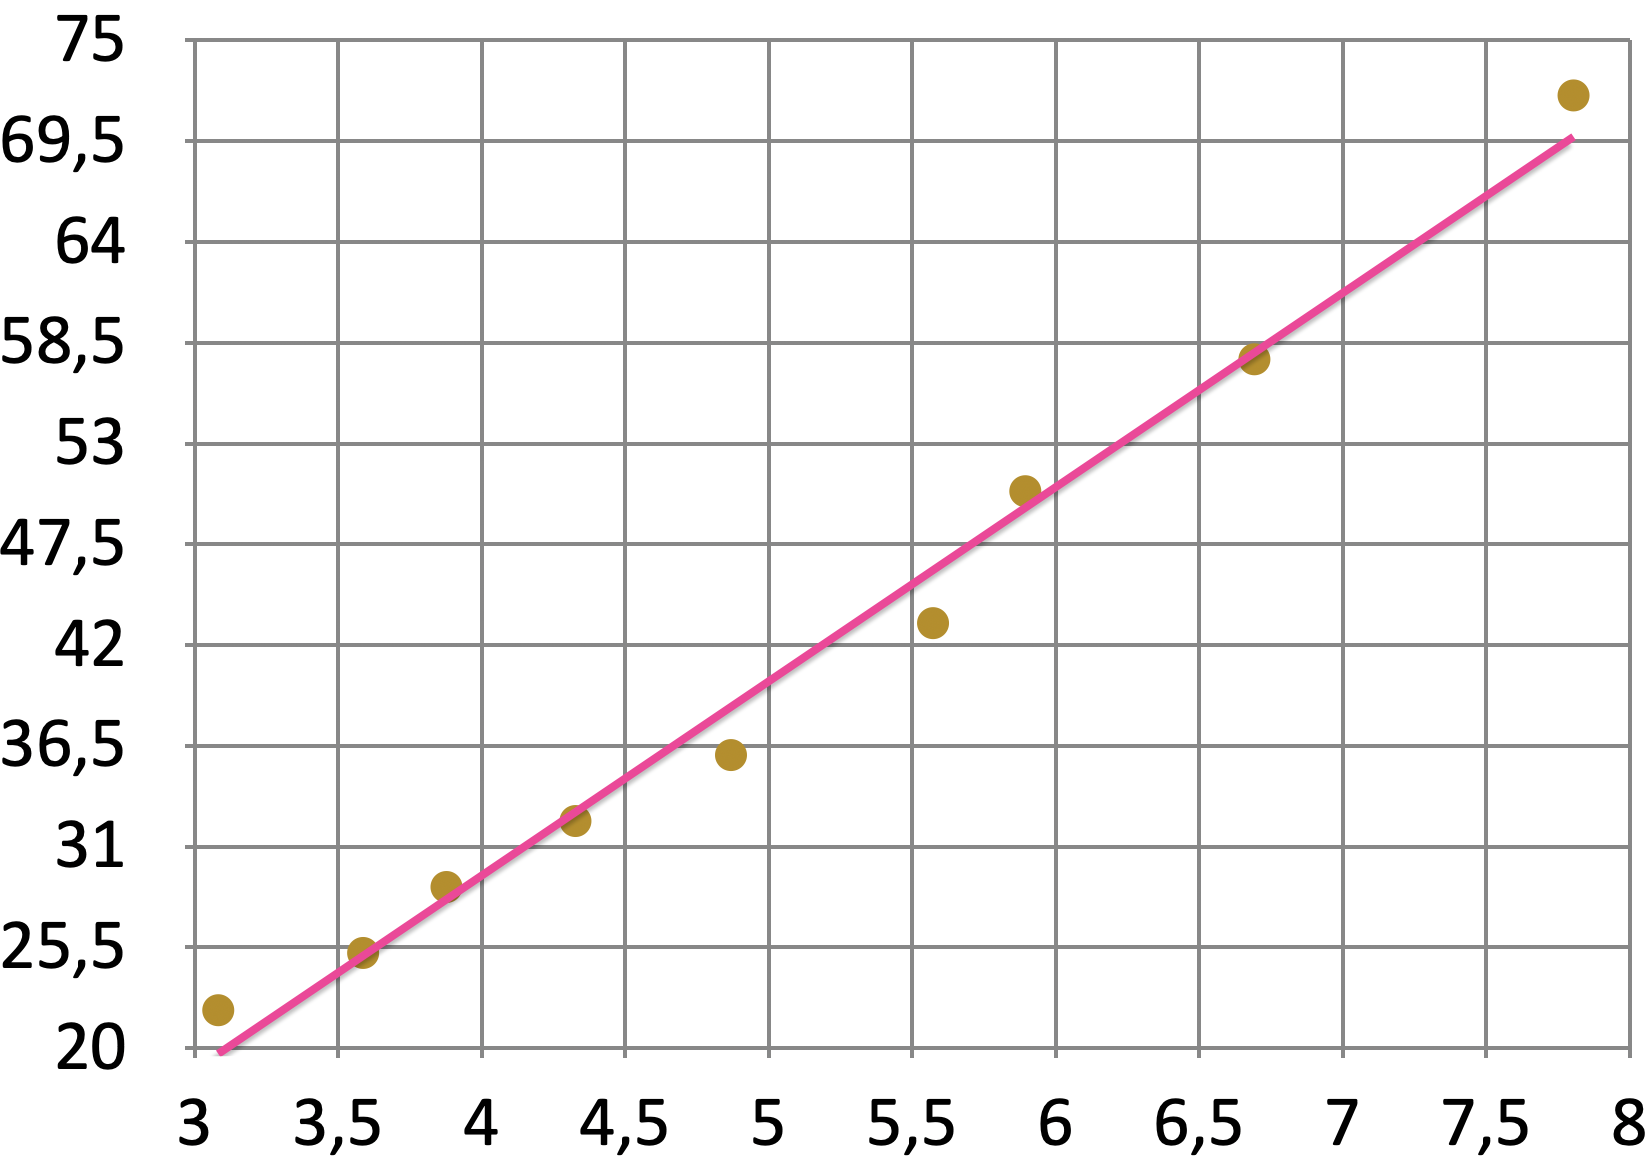
\includegraphics[width=50mm]{p5.png}
		\caption{Схема ионизационной лампы ЛТ-2}
		\label{fig:лампа}
	\end{center}
\end{wrapfigure}

\textit{Ионизационный манометр.} Схема ионизационного манометра изображения на рис. 3. Он представляет собой трехэлектродную лампу. Электроны испускаются раскалённым катодом и увлекаются электрическим полем к аноду, имеющему вид редкой спирали. Проскакивая за её витки, электроны замедляются полем коллектора и возвращаются к аноду. Прежде чем осесть на аноде, они успевают много раз пересечь пространство между катодом и коллектором. На своём пути электроны ионизуют молекулы газа. Ионы, образовавшиеся между анодом и коллектором, притягиваются полем коллектора и определяют его ток.
Накалённый катод ионизационного манометра перегорает, если давление в системе превышает $10^{-3}$ торр, поэтому перед его включением необходимо проверить давление термопарным манометром.

\subsection{Процесс откачки}
Опишем процесс откачки математически:
Пусть W --- объем газа, удаляемого из сосуда при данном давлении за единицу времени, $Q_i$ для различных значений i обозначим различные притоки газа в сосуд (в единицах PV), такие как течи извне $Q_\text{и}$, десорбция с поверхностей внутри сосуда $Q_\text{д}$, обратный ток через насос $Q_\text{н}$. Тогда, приравнивая убыль газа из сосуда (с точностью до $RT/\mu$) в единицу времени $-VdP$ и сумму перечисленных токов? имеем:
 \begin{equation}
 	-VdP = (PW - \sum_i Q_i)dt
 \end{equation}
 При достижении предельного вакуума устанавливается давление $P_{\text{пр}}$, и $dP = 0$. Тогда
 \begin{equation}
 	 W = ( \sum_i Q_i )/P_{\text{пр}}
 \end{equation}
 Поскольку обычно $Q_\text{и}$ постоянно, а $Q_\text{н}$ и $Q_\text{д}$ слабо зависят от времени, также считая постоянной W, можем проинтегрировать (1) и получить:
 \begin{equation}
 	P - P_{\text{пр}} = (P_0 - P_{\text{пр}})\exp(-\frac{W}{V}t)
 \end{equation}
Полная скорость откачки $W$, собственная скорость откачки насоса $W_{\text{н}}$ и проводимости элементов системы $C_1, C_2,...$ соотносятся согласно формуле (4), и это учтено в конструкции установки.
 \begin{equation}
 \frac{1}{W} = \frac{1}{W} + \frac{1}{C_1} + \frac{1}{C_2} + ...
\end{equation}

Характер течения газа существенно зависит от соотношения между размерами системы и длиной свободного пробега молекул. При атмосферном и форвакуумном давлениях  длина свободного пробега меньше диаметра трубок, и течение газа определяется его вязкостью, т.е. взаимодействием молекул. При высоком вакууме течение существеннее определяется взаимодействием со стенками \\
Для количества газа, протекающего через трубу длины $l$ и радиуса $r$ в условиях высокого вакуума, справедлива формула:
\begin{equation}
	\frac{d(PV)}{dt} = \frac{4}{3}r^3\sqrt{\frac{2\pi RT}{\mu}}\frac{P_2 - P_1}{l}
\end{equation}
Если труба соединяет насос установку, то давлением $P_1$ у насоса можно пренебречь. Давление в сосуде $P = P_2$. Тогда имеем:
\begin{equation}
C_\text{тр} = \left(\frac{dV}{dt}\right)_\text{тр} = \frac{4r^3}{3l}\sqrt{\frac{2\pi RT}{\mu}}
\end{equation}
Для пропускной способности отверстий имеется формула
\begin{equation}
C_\text{отв} = \left(\frac{dV}{dt}\right)_\text{отв} = S\frac{\bar{\upsilon}}{4}
\end{equation}
